\documentclass[article]{abntex2} 
\usepackage{graphicx}
\usepackage{url}
\usepackage{blindtext}
\usepackage{tabu}
\title{Relatorio 1\\Fisica Experimental 3 - Turma E} 
\author{Grupo 2
    \\Luis Humberto Chaves Senno - 180053922
    \\Marcos Eduardo Monteiro Junqueira - 180023691
    \\Emanuel Couto Brenag - 190057131}      
\date{27 de Março, 2019}   

\begin{document}            
\maketitle   
\newpage 
\section{Introdução}   
\subsection{Introdução}
As Leis de Kirchhoff são aplicadas em circuitos elétricos 
que apresentam mais de um resistor, estando os outros 
em série ou em paralelo com o primeiro. 

Para entender as leis de Kirchhoff, é essencial
 o entendimento de outros dois conceitos, os Nós e as Malhas:

Nó: é um ponto onde três (ou mais) condutores são ligados.

Malha: é qualquer caminho condutor fechado.

A primeira lei de Kirchhoff também é conhecida como Lei dos Nós. Ela diz que em qualquer nó, a soma de correntes que apontam para fora dele é igual a soma das correntes que chegam. Ela confirma que não há cargas acumuladas nos Nós. 
(Fórmula do somatório dos i’s=0)

A segunda lei de Kirchhoff é conhecida como Lei das Malhas. Ela diz que a soma das forças eletromotrizes de uma malha é igual a soma das quedas de potencial da mesma.
(Somatório de E = Somatório de R.i).
\subsection{Materiais}
\begin{itemize}
    \item 1 Resistor de $390\Omega(R_1)$
    \item 1 Resistor de $1k\Omega(R_2)$
    \item 1 Resistor de $1M\Omega(R_3)$
    \item 1 Fonte Controlada de Tensão/Corrente
    \item 2 Multímetros de Bancada digitais modelo EEL-8002
\end{itemize}
\subsection{Objetivo}
O experimento tem como objetivo a familiarização
 dos conceitos básicos de montagem e análise de um
  circuito elétrico e utilização de um multímetro. 
  Além disso serão utilizados esses conhecimentos
   para verificação das duas leis de Kirchoff,
    fundamentais para a análise de circuitos.
\section{Dados Experimentais}
\subsection{Parte I - Uso dos Multímetros e Resistencias Internas}
%tabela1
\begin{table}[htb]
\begin{center}
\caption{Voltagem e Corrente no Resistor 1($390\Omega$)}
\begin{tabular}{ |c|c|c| }
    \hline
    $V_f$ &$V$ &$I$ \\
    \hline
    $4,0 \pm 0,1V$ &$3,962 \pm 0,001V$ &$10,492 \pm 0,001mA$ \\
    \hline
    $8,0 \pm 0,1V$ &$8,090 \pm 0,001V$ &$21,44 \pm 0,01mA$ \\
    \hline
    $12,0 \pm 0,1V$ &$12,125 \pm 0,001V$ &$32,10 \pm 0,01mA$ \\
    \hline
    $16,0 \pm 0,1V$ &$16,163 \pm 0,001V$ &$42,72 \pm 0,01mA$ \\
    \hline
    $20,0 \pm 0,1V$ &$20,12 \pm 0,01V$ &$53,23 \pm 0,01mA$ \\
    \hline
\end{tabular}
\end{center}
\end{table}
%tabela 2
\begin{table}[htb]
\begin{center}
\caption{Voltagem e Corrente no Resistor 2($1k\Omega$)}
\begin{tabular}{ |c|c|c| }
        \hline
        $V_f$ &$V$ &$I$ \\
        \hline
        $4,0 \pm 0,1V$ &$4,003 \pm 0,001V$ &$3,874 \pm 0,001mA$ \\
        \hline
        $8,0 \pm 0,1V$ &$8,030 \pm 0,001V$ &$7,765 \pm 0,001mA$ \\
        \hline
        $12,0 \pm 0,1V$ &$12,053 \pm 0,001V$ &$11,665 \pm 0,001mA$ \\
        \hline
        $16,0 \pm 0,1V$ &$16,038 \pm 0,001V$ &$15,515\pm 0,001mA$ \\
        \hline
        $20,0 \pm 0,1V$ &$19,986 \pm 0,001V$ &$19,333 \pm 0,001mA$ \\
        \hline
\end{tabular}
\end{center}
\end{table}
%tabela 3
\begin{table}[htb]
\begin{center}
\caption{Voltagem e Corrente no Resistor 3($1M\Omega$)}
\begin{tabular}{ |c|c|c| }
        \hline
        $V_f$ &$V$ &$I$ \\
        \hline
        $4,0 \pm 0,1V$ &$4,107 \pm 0,001V$ &$0,004 \pm 0,001mA$ \\
        \hline
        $8,0 \pm 0,1V$ &$8,085 \pm 0,001V$ &$0,009 \pm 0,001mA$ \\
        \hline
        $12,0 \pm 0,1V$ &$12,134 \pm 0,001V$ &$0,014 \pm 0,001mA$ \\
        \hline
        $16,0 \pm 0,1V$ &$16,184 \pm 0,001V$ &$0,018 \pm 0,001mA$ \\
        \hline
        $20,0 \pm 0,1V$ &$20,25 \pm 0,01V$ &$0,023 \pm 0,001mA$ \\
        \hline
\end{tabular}
\end{center}
\end{table}
%tabela 4
\begin{table}[htb]
\begin{center}
\caption{Voltagem e Corrente no Resistor 3($1M\Omega$) com Amperímetro Reposicionado}
\begin{tabular}{ |c|c|c| }
            \hline
            $V_f$ &$V$ &$I$ \\
            \hline
            $4,0 \pm 0,1V$ &$4,068 \pm 0,001V$ &$0,003 \pm 0,001mA$ \\
            \hline
            $8,0 \pm 0,1V$ &$8,100 \pm 0,001V$ &$0,007 \pm 0,001mA$ \\
            \hline
            $12,0 \pm 0,1V$ &$12,120 \pm 0,001V$ &$0,012 \pm 0,001mA$ \\
            \hline
            $16,0 \pm 0,1V$ &$16,219 \pm 0,001V$ &$0,016 \pm 0,001mA$ \\
            \hline
            $20,0 \pm 0,1V$ &$20,22 \pm 0,01V$ &$0,020 \pm 0,001mA$ \\
            \hline
\end{tabular}
\end{center}
\end{table}
\newpage
Onde:
\newline

$V_f =$ Valor da Voltagem Marcado na Fonte

$V =$ Valor da Voltagem Marcado pelo Multímetro

$I =$ Valor da Corrente Marcado pelo Multímetro
\newline   

As tabelas 1,2,3 foram feitos com dados obtidos a partir de medições
no circuito a seguir:
\begin{figure}[htb]
\begin{center}
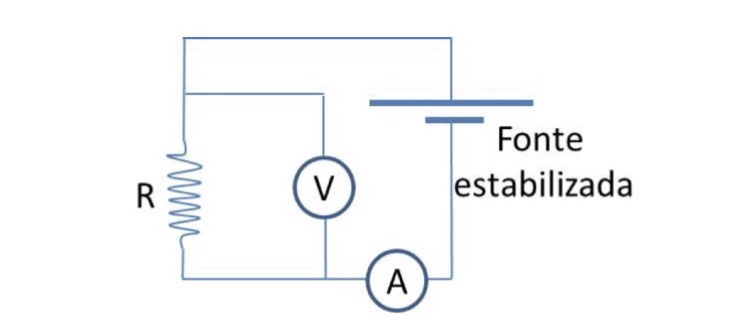
\includegraphics[scale=0.4]{circuito1.jpg} 
\end{center}
\end{figure}

Já os dados da tabela 4 foram obtidos do seguinte circuito:
\newpage
\begin{figure}[htb]
\begin{center}
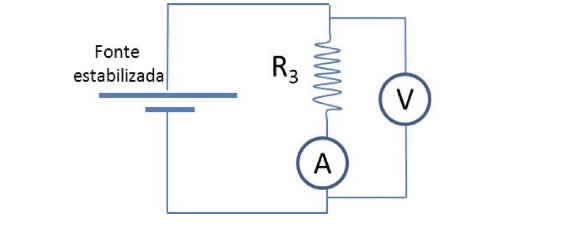
\includegraphics[scale=0.5]{circuito5.jpg} 
\end{center}
\end{figure}
\subsection{Parte II - Lei das Malhas}
%tabela5
\begin{table}[htb]
\begin{center}
\caption{Resistores em Serie}
\begin{tabular}{  |c|c|c|c|c| }
    \hline
    $V_f$ &$V_{R1}$ &$V_{R2}$ &$V_{ab}$ &$I$ \\
    \hline
    $10,0 \pm 0,1V$ &$2,618 \pm 0,001V$ &$7,380 \pm 0,001V$ &$10,071 \pm 0,001V$ &$7,134 \pm 0,001mA$ \\
    \hline
    $20,0 \pm 0,1V$ &$5,369 \pm 0,001V$ &$14,701 \pm 0,001V$ &$20,07 \pm 0,01V$ &$14,213 \pm 0,001mA$ \\
    \hline
\end{tabular}
\end{center}
\end{table}
Onde:
\newline

$V_f =$ Valor da Voltagem Marcado na Fonte

$V_{R1} =$ Valor da Voltagem Marcado pelo Multímetro
 em Paralelo com R1

$V_{R2} =$ Valor da Voltagem Marcado pelo Multímetro 
em Paralelo com R2

$V_{R2} =$ Valor da Voltagem Marcado pelo Multímetro
 em Paralelo com R1 e R2 posicionados em série

$I =$ Valor da Corrente Marcado pelo Multímetro
\newline   

As medicçõs para a tabela 5 foram feitas alternando o Voltímetro 
de posição conforme os  circuitos abaixo:
\begin{figure}[htb]
\begin{center}
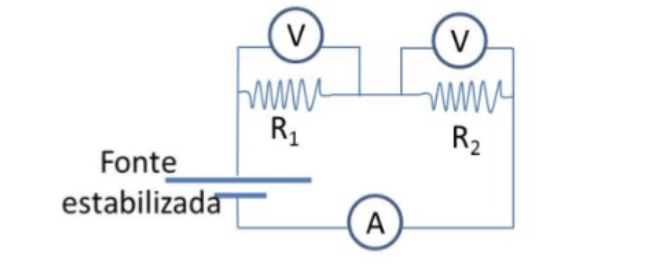
\includegraphics[scale=0.4]{circuito2.jpg} 
\end{center}
\end{figure}
\begin{figure}[htb]
\begin{center}
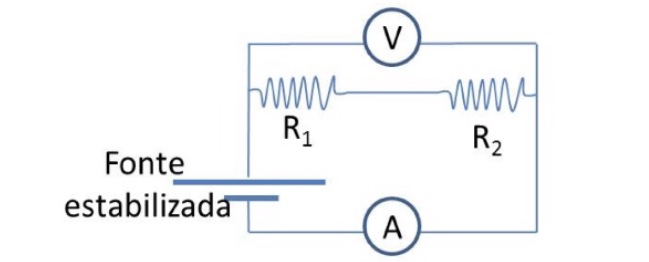
\includegraphics[scale=0.4]{circuito3.jpg} 
\end{center}
\end{figure}
\newpage
\subsection{Parte III - Lei do Nós}
%tabela 6
\begin{table}[htb]
\begin{center}
\caption{Resistores em Paralelo}
\begin{tabular}{  |c|c|c|c|c| }
    \hline
    $V_f$ &$I_{R1}$ &$I_{R2}$ &$I_{ab}$ &$V_{ab}$ \\
    \hline
    $10,0 \pm 0,1V$ &$26,67 \pm 0,01mA$ &$9,672 \pm 0,001mA$ &$36,45 \pm 0,01mA$ &$10,073 \pm 0,001V$  \\
    \hline
    $20,0 \pm 0,1V$ &$53,28 \pm 0,01mA$ &$19,364 \pm 0,001mA$ &$75,58 \pm 0,01mA$ &$20,10 \pm 0,01V$  \\
    \hline
\end{tabular}
\end{center}
\end{table}
Onde:
\newline

$V_f =$ Valor da Voltagem Marcado na Fonte

$I_{R1} =$ Valor da Corrente Marcado pelo Multímetro
 em Série com R1

$I_{R2} =$ Valor da Corrente Marcado pelo Multímetro 
em Série com R2

$I_{ab} =$ Valor da Corrente Marcado pelo Multímetro
 em Série com R1 e R2 posicionados em Paralelo

$V_{ab} =$ Valor da Voltagem Marcado pelo Multímetro
em Paralelo com R1 e R2 posicionados em Paralelo
\newline 

Ao mudar a posição do Amperímetro de acordo com o circuito abaixo
foi possível a obtenção dos dados da tabela acima.
\begin{figure}[htb]
\begin{center}
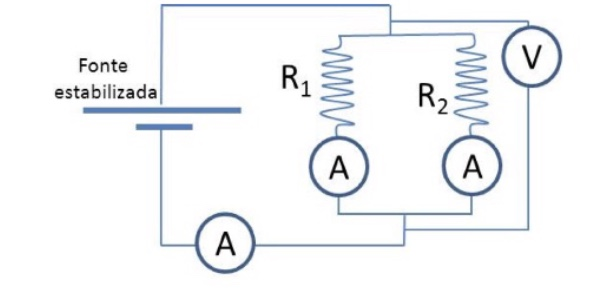
\includegraphics[scale=0.45]{circuito4.jpg} 
\end{center}
\end{figure}
\newpage

\section{Análise dos Dados}
\subsection{Parte I - Uso dos Multímetros e Resistências Internas}
%grafico
\begin{figure}[htb]
\begin{center}
\caption{Tensão por Corrente nos Resistores 1 e 2}
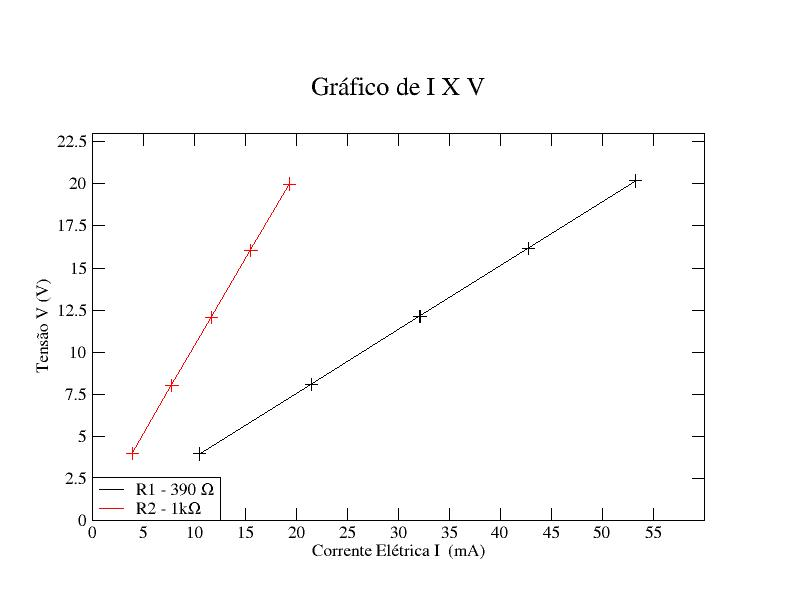
\includegraphics[scale=0.7]{grafico1,1.jpg} 
\end{center}
\end{figure}

\newpage

\begin{figure}[htb]
\begin{center}
\caption{Tensão por Corrente no Resistor 3}
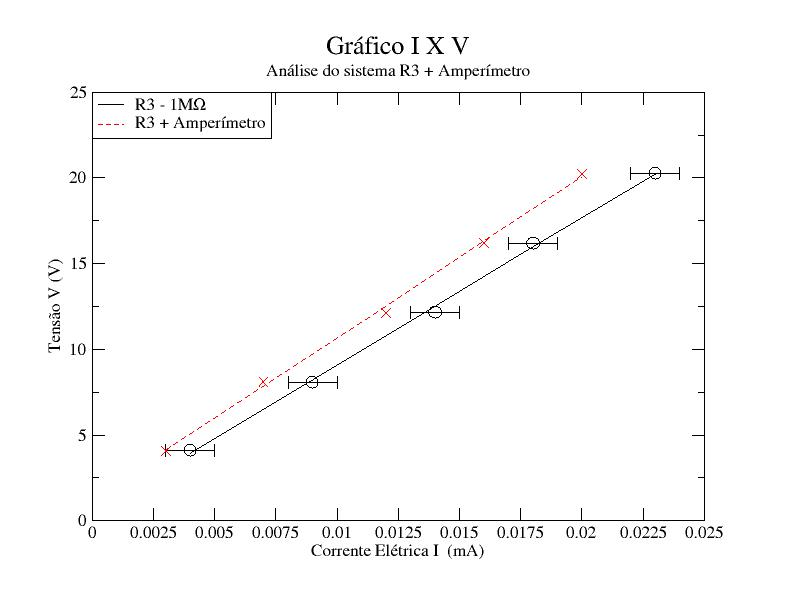
\includegraphics[scale=0.7]{grafico1,2.jpg} 
\end{center}
\end{figure}

\section{Conclusão}

A partir dos valores que foram obtidos experimentalmente,
 realizando os cálculos da lei dos nós, verifica-se que a soma 
 das correntes que saem e que entram resulta em um número
  extremamente próximo de 0, numa margem coberta pelo
   erro experimental. Também verificou-se que a soma
    das eletromotrizes é igual a soma das quedas de
     tensão (R.i), podendo assim confirmar e afirmar
      que as duas leis de Kirchhoff são válidas.

\section{Bibliografia}
Todas as imagens de circuitos foram retiradas diretamente
do roteiro do experimento, localizado 
no ambiente virtual do Departamento de Fisica da UnB.
\newline

\url{https://ifserv.fis.unb.br/moodle/}

\url{https://pt.wikipedia.org/wiki/Leis_de_Kirchhoff}

Halliday, Resnick, Krane. Física 3, LTC, 5a Ed., 2004
\end{document}